% Options for packages loaded elsewhere
% Options for packages loaded elsewhere
\PassOptionsToPackage{unicode}{hyperref}
\PassOptionsToPackage{hyphens}{url}
\PassOptionsToPackage{dvipsnames,svgnames,x11names}{xcolor}
%
\documentclass[
]{article}
\usepackage{xcolor}
\usepackage[margin=1in]{geometry}
\usepackage{amsmath,amssymb}
\setcounter{secnumdepth}{5}
\usepackage{iftex}
\ifPDFTeX
  \usepackage[T1]{fontenc}
  \usepackage[utf8]{inputenc}
  \usepackage{textcomp} % provide euro and other symbols
\else % if luatex or xetex
  \usepackage{unicode-math} % this also loads fontspec
  \defaultfontfeatures{Scale=MatchLowercase}
  \defaultfontfeatures[\rmfamily]{Ligatures=TeX,Scale=1}
\fi
\usepackage{lmodern}
\ifPDFTeX\else
  % xetex/luatex font selection
\fi
% Use upquote if available, for straight quotes in verbatim environments
\IfFileExists{upquote.sty}{\usepackage{upquote}}{}
\IfFileExists{microtype.sty}{% use microtype if available
  \usepackage[]{microtype}
  \UseMicrotypeSet[protrusion]{basicmath} % disable protrusion for tt fonts
}{}
\makeatletter
\@ifundefined{KOMAClassName}{% if non-KOMA class
  \IfFileExists{parskip.sty}{%
    \usepackage{parskip}
  }{% else
    \setlength{\parindent}{0pt}
    \setlength{\parskip}{6pt plus 2pt minus 1pt}}
}{% if KOMA class
  \KOMAoptions{parskip=half}}
\makeatother
% Make \paragraph and \subparagraph free-standing
\makeatletter
\ifx\paragraph\undefined\else
  \let\oldparagraph\paragraph
  \renewcommand{\paragraph}{
    \@ifstar
      \xxxParagraphStar
      \xxxParagraphNoStar
  }
  \newcommand{\xxxParagraphStar}[1]{\oldparagraph*{#1}\mbox{}}
  \newcommand{\xxxParagraphNoStar}[1]{\oldparagraph{#1}\mbox{}}
\fi
\ifx\subparagraph\undefined\else
  \let\oldsubparagraph\subparagraph
  \renewcommand{\subparagraph}{
    \@ifstar
      \xxxSubParagraphStar
      \xxxSubParagraphNoStar
  }
  \newcommand{\xxxSubParagraphStar}[1]{\oldsubparagraph*{#1}\mbox{}}
  \newcommand{\xxxSubParagraphNoStar}[1]{\oldsubparagraph{#1}\mbox{}}
\fi
\makeatother

\usepackage{color}
\usepackage{fancyvrb}
\newcommand{\VerbBar}{|}
\newcommand{\VERB}{\Verb[commandchars=\\\{\}]}
\DefineVerbatimEnvironment{Highlighting}{Verbatim}{commandchars=\\\{\}}
% Add ',fontsize=\small' for more characters per line
\usepackage{framed}
\definecolor{shadecolor}{RGB}{241,243,245}
\newenvironment{Shaded}{\begin{snugshade}}{\end{snugshade}}
\newcommand{\AlertTok}[1]{\textcolor[rgb]{0.68,0.00,0.00}{#1}}
\newcommand{\AnnotationTok}[1]{\textcolor[rgb]{0.37,0.37,0.37}{#1}}
\newcommand{\AttributeTok}[1]{\textcolor[rgb]{0.40,0.45,0.13}{#1}}
\newcommand{\BaseNTok}[1]{\textcolor[rgb]{0.68,0.00,0.00}{#1}}
\newcommand{\BuiltInTok}[1]{\textcolor[rgb]{0.00,0.23,0.31}{#1}}
\newcommand{\CharTok}[1]{\textcolor[rgb]{0.13,0.47,0.30}{#1}}
\newcommand{\CommentTok}[1]{\textcolor[rgb]{0.37,0.37,0.37}{#1}}
\newcommand{\CommentVarTok}[1]{\textcolor[rgb]{0.37,0.37,0.37}{\textit{#1}}}
\newcommand{\ConstantTok}[1]{\textcolor[rgb]{0.56,0.35,0.01}{#1}}
\newcommand{\ControlFlowTok}[1]{\textcolor[rgb]{0.00,0.23,0.31}{\textbf{#1}}}
\newcommand{\DataTypeTok}[1]{\textcolor[rgb]{0.68,0.00,0.00}{#1}}
\newcommand{\DecValTok}[1]{\textcolor[rgb]{0.68,0.00,0.00}{#1}}
\newcommand{\DocumentationTok}[1]{\textcolor[rgb]{0.37,0.37,0.37}{\textit{#1}}}
\newcommand{\ErrorTok}[1]{\textcolor[rgb]{0.68,0.00,0.00}{#1}}
\newcommand{\ExtensionTok}[1]{\textcolor[rgb]{0.00,0.23,0.31}{#1}}
\newcommand{\FloatTok}[1]{\textcolor[rgb]{0.68,0.00,0.00}{#1}}
\newcommand{\FunctionTok}[1]{\textcolor[rgb]{0.28,0.35,0.67}{#1}}
\newcommand{\ImportTok}[1]{\textcolor[rgb]{0.00,0.46,0.62}{#1}}
\newcommand{\InformationTok}[1]{\textcolor[rgb]{0.37,0.37,0.37}{#1}}
\newcommand{\KeywordTok}[1]{\textcolor[rgb]{0.00,0.23,0.31}{\textbf{#1}}}
\newcommand{\NormalTok}[1]{\textcolor[rgb]{0.00,0.23,0.31}{#1}}
\newcommand{\OperatorTok}[1]{\textcolor[rgb]{0.37,0.37,0.37}{#1}}
\newcommand{\OtherTok}[1]{\textcolor[rgb]{0.00,0.23,0.31}{#1}}
\newcommand{\PreprocessorTok}[1]{\textcolor[rgb]{0.68,0.00,0.00}{#1}}
\newcommand{\RegionMarkerTok}[1]{\textcolor[rgb]{0.00,0.23,0.31}{#1}}
\newcommand{\SpecialCharTok}[1]{\textcolor[rgb]{0.37,0.37,0.37}{#1}}
\newcommand{\SpecialStringTok}[1]{\textcolor[rgb]{0.13,0.47,0.30}{#1}}
\newcommand{\StringTok}[1]{\textcolor[rgb]{0.13,0.47,0.30}{#1}}
\newcommand{\VariableTok}[1]{\textcolor[rgb]{0.07,0.07,0.07}{#1}}
\newcommand{\VerbatimStringTok}[1]{\textcolor[rgb]{0.13,0.47,0.30}{#1}}
\newcommand{\WarningTok}[1]{\textcolor[rgb]{0.37,0.37,0.37}{\textit{#1}}}

\usepackage{longtable,booktabs,array}
\usepackage{calc} % for calculating minipage widths
% Correct order of tables after \paragraph or \subparagraph
\usepackage{etoolbox}
\makeatletter
\patchcmd\longtable{\par}{\if@noskipsec\mbox{}\fi\par}{}{}
\makeatother
% Allow footnotes in longtable head/foot
\IfFileExists{footnotehyper.sty}{\usepackage{footnotehyper}}{\usepackage{footnote}}
\makesavenoteenv{longtable}
\usepackage{graphicx}
\makeatletter
\newsavebox\pandoc@box
\newcommand*\pandocbounded[1]{% scales image to fit in text height/width
  \sbox\pandoc@box{#1}%
  \Gscale@div\@tempa{\textheight}{\dimexpr\ht\pandoc@box+\dp\pandoc@box\relax}%
  \Gscale@div\@tempb{\linewidth}{\wd\pandoc@box}%
  \ifdim\@tempb\p@<\@tempa\p@\let\@tempa\@tempb\fi% select the smaller of both
  \ifdim\@tempa\p@<\p@\scalebox{\@tempa}{\usebox\pandoc@box}%
  \else\usebox{\pandoc@box}%
  \fi%
}
% Set default figure placement to htbp
\def\fps@figure{htbp}
\makeatother





\setlength{\emergencystretch}{3em} % prevent overfull lines

\providecommand{\tightlist}{%
  \setlength{\itemsep}{0pt}\setlength{\parskip}{0pt}}



 


\makeatletter
\@ifpackageloaded{caption}{}{\usepackage{caption}}
\AtBeginDocument{%
\ifdefined\contentsname
  \renewcommand*\contentsname{Table of contents}
\else
  \newcommand\contentsname{Table of contents}
\fi
\ifdefined\listfigurename
  \renewcommand*\listfigurename{List of Figures}
\else
  \newcommand\listfigurename{List of Figures}
\fi
\ifdefined\listtablename
  \renewcommand*\listtablename{List of Tables}
\else
  \newcommand\listtablename{List of Tables}
\fi
\ifdefined\figurename
  \renewcommand*\figurename{Figure}
\else
  \newcommand\figurename{Figure}
\fi
\ifdefined\tablename
  \renewcommand*\tablename{Table}
\else
  \newcommand\tablename{Table}
\fi
}
\@ifpackageloaded{float}{}{\usepackage{float}}
\floatstyle{ruled}
\@ifundefined{c@chapter}{\newfloat{codelisting}{h}{lop}}{\newfloat{codelisting}{h}{lop}[chapter]}
\floatname{codelisting}{Listing}
\newcommand*\listoflistings{\listof{codelisting}{List of Listings}}
\makeatother
\makeatletter
\makeatother
\makeatletter
\@ifpackageloaded{caption}{}{\usepackage{caption}}
\@ifpackageloaded{subcaption}{}{\usepackage{subcaption}}
\makeatother
\usepackage{bookmark}
\IfFileExists{xurl.sty}{\usepackage{xurl}}{} % add URL line breaks if available
\urlstyle{same}
\hypersetup{
  pdftitle={Lecture - Lecture Notes},
  colorlinks=true,
  linkcolor={blue},
  filecolor={Maroon},
  citecolor={Blue},
  urlcolor={Blue},
  pdfcreator={LaTeX via pandoc}}


\title{Lecture - Lecture Notes}
\author{}
\date{}
\begin{document}
\maketitle

\renewcommand*\contentsname{Table of contents}
{
\hypersetup{linkcolor=}
\setcounter{tocdepth}{3}
\tableofcontents
}

\section{Advanced Machine Learning: Deep Neural
Networks}\label{advanced-machine-learning-deep-neural-networks}

\textbf{Author}: Prof.~AI Researcher\\
\textbf{Date}: September 2025\\
\textbf{Institute}: University of Pisa - Master in AI

\subsection{Overview}\label{overview}

Today we'll explore the cutting-edge world of deep neural networks,
covering:

\begin{itemize}
\tightlist
\item
  Mathematical foundations of deep learning
\item
  Advanced architectures and their applications
\item
  Optimization techniques and regularization
\item
  Practical implementation strategies
\end{itemize}

This lecture builds on previous knowledge of basic machine learning
concepts. Students should be familiar with linear algebra, calculus.

Probability theory. we'll dive deep into the theoretical foundations
while maintaining practical relevance through real-world examples.

The lecture is structured to progressively build complexity, starting
from fundamental concepts and moving toward state-of-the-art techniques
used in modern AI research.

\subsection{The Universal Approximation
Theorem}\label{the-universal-approximation-theorem}

Neural networks are \textbf{universal function approximators}:

\[f(x) = \sum_{i=1}^{n} w_i \sigma(W_i^T x + b_i)\]

Where: - \(\sigma\) is the activation function - \(W_i\) are weight
matrices\\
- \(b_i\) are bias vectors - \(n\) is the number of hidden units

\subsection{The Universal Approximation Theorem
(2)}\label{the-universal-approximation-theorem-2}

The Universal Approximation Theorem, first proven by Cybenko in 1989,
states that a feedforward network with a single hidden layer containing
a finite number of neurons can approximate any continuous function on
compact subsets of \(\mathbb{R}^n\) to arbitrary accuracy.

\subsection{The Universal Approximation Theorem
(3)}\label{the-universal-approximation-theorem-3}

This is a profound theoretical result that provides the mathematical
foundation for why neural networks work. However, the theorem doesn't
tell us: 1. How many neurons we need 2. How to find the optimal weights
3. Whether the approximation generalizes to unseen data

In practice, deeper networks often achieve better performance with fewer
parameters than very wide shallow networks.

\begin{figure}[H]

{\centering \pandocbounded{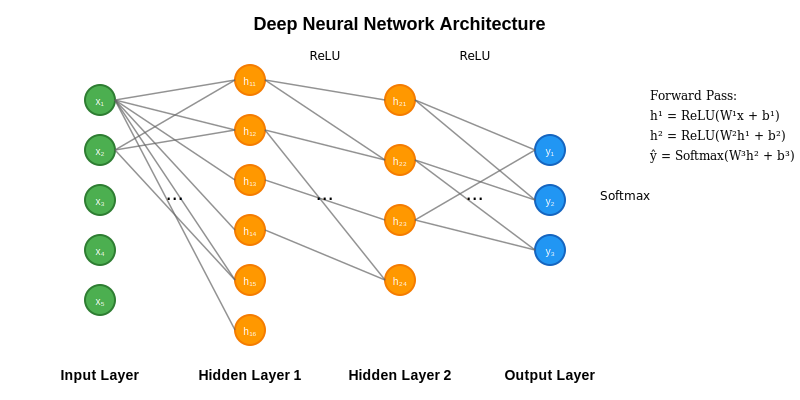
\includegraphics[keepaspectratio]{lecture_notes_files/mediabag/figures/neural_network.pdf}}

}

\caption{Neural Network Architecture}

\end{figure}%

\subsection{Deep Learning Mathematics}\label{deep-learning-mathematics}

\subsubsection{Gradient Computation via
Backpropagation}\label{gradient-computation-via-backpropagation}

The chain rule enables efficient gradient computation:

\[\frac{\partial L}{\partial W^{(l)}} = \frac{\partial L}{\partial z^{(l+1)}} \cdot \frac{\partial z^{(l+1)}}{\partial a^{(l)}} \cdot \frac{\partial a^{(l)}}{\partial W^{(l)}}\]

\subsubsection{Loss Function Landscape}\label{loss-function-landscape}

For classification with \(C\) classes:

\[L_{CE} = -\sum_{i=1}^{N} \sum_{c=1}^{C} y_{ic} \log(\hat{y}_{ic})\]

Backpropagation is the heart of neural network training. The algorithm
efficiently computes gradients by applying the chain rule recursively
from the output layer back to the input layer.

Key insights about the gradient computation:

\begin{enumerate}
\def\labelenumi{\arabic{enumi}.}
\tightlist
\item
  \textbf{Computational Graph}: We can represent the forward pass as a
  computational graph where each node represents an operation.
\end{enumerate}

\subsubsection{Loss Function Landscape
(2)}\label{loss-function-landscape-2}

\begin{enumerate}
\def\labelenumi{\arabic{enumi}.}
\setcounter{enumi}{1}
\item
  \textbf{Dynamic Programming}: Backpropagation is essentially dynamic
  programming applied to gradient computation, avoiding redundant
  calculations.
\item
  \textbf{Vanishing Gradients}: In very deep networks, gradients can
  become exponentially small, making training difficult. This led to
  innovations like:

  \begin{itemize}
  \tightlist
  \item
    Skip connections (ResNet)
  \item
    Better activation functions (ReLU, Swish)
  \item
    Normalization techniques (BatchNorm, LayerNorm)
  \end{itemize}
\item
  \textbf{Exploding Gradients}: Conversely, gradients can also explode,
  leading to unstable training. Gradient clipping is a common solution.
\end{enumerate}

\subsubsection{Loss Function Landscape
(3)}\label{loss-function-landscape-3}

The cross-entropy loss function is particularly well-suited for
classification because: - It's convex in the final layer weights - It
provides strong gradients when predictions are confident but wrong - It
naturally handles the probabilistic interpretation of softmax outputs

\subsection{Advanced Architectures}\label{advanced-architectures}

\subsubsection{Convolutional Neural Networks
(CNNs)}\label{convolutional-neural-networks-cnns}

\begin{Shaded}
\begin{Highlighting}[]


\OperatorTok{\textless{}!{-}{-}}\NormalTok{ Transition: Moving to }\BuiltInTok{next}\NormalTok{ topic }\OperatorTok{{-}{-}\textgreater{}}



\CommentTok{\# Modern CNN block with residual connections}
\KeywordTok{class}\NormalTok{ ResidualBlock(nn.Module):}
    \KeywordTok{def} \FunctionTok{\_\_init\_\_}\NormalTok{(}\VariableTok{self}\NormalTok{, channels):}
        \BuiltInTok{super}\NormalTok{().}\FunctionTok{\_\_init\_\_}\NormalTok{()}
        \VariableTok{self}\NormalTok{.conv1 }\OperatorTok{=}\NormalTok{ nn.Conv2d(channels, channels, }\DecValTok{3}\NormalTok{, padding}\OperatorTok{=}\DecValTok{1}\NormalTok{)}
        \VariableTok{self}\NormalTok{.bn1 }\OperatorTok{=}\NormalTok{ nn.BatchNorm2d(channels)}
        \VariableTok{self}\NormalTok{.conv2 }\OperatorTok{=}\NormalTok{ nn.Conv2d(channels, channels, }\DecValTok{3}\NormalTok{, padding}\OperatorTok{=}\DecValTok{1}\NormalTok{)}
        \VariableTok{self}\NormalTok{.bn2 }\OperatorTok{=}\NormalTok{ nn.BatchNorm2d(channels)}
        \VariableTok{self}\NormalTok{.relu }\OperatorTok{=}\NormalTok{ nn.ReLU(inplace}\OperatorTok{=}\VariableTok{True}\NormalTok{)}
        
\end{Highlighting}
\end{Shaded}

\subsubsection{Code (continued)}\label{code-continued}

\begin{Shaded}
\begin{Highlighting}[]
    \KeywordTok{def}\NormalTok{ forward(}\VariableTok{self}\NormalTok{, x):}
\NormalTok{        identity }\OperatorTok{=}\NormalTok{ x}
\NormalTok{        out }\OperatorTok{=} \VariableTok{self}\NormalTok{.relu(}\VariableTok{self}\NormalTok{.bn1(}\VariableTok{self}\NormalTok{.conv1(x)))}
\NormalTok{        out }\OperatorTok{=} \VariableTok{self}\NormalTok{.bn2(}\VariableTok{self}\NormalTok{.conv2(out))}
\NormalTok{        out }\OperatorTok{+=}\NormalTok{ identity  }\CommentTok{\# Skip connection}
        \ControlFlowTok{return} \VariableTok{self}\NormalTok{.relu(out)}
\end{Highlighting}
\end{Shaded}

\subsubsection{Attention Mechanisms}\label{attention-mechanisms}

The attention weight computation:

\[\text{Attention}(Q, K, V) = \text{softmax}\left(\frac{QK^T}{\sqrt{d_k}}\right)V\]

Where: - \(Q\) is the query matrix - \(K\) is the key matrix\\
- \(V\) is the value matrix - \(d_k\) is the key dimension

Attention mechanisms have revolutionized deep learning, particularly in
natural language processing and computer vision. The key insight is that
not all parts of the input are equally important for making predictions.

\subsubsection{Attention Mechanisms (2)}\label{attention-mechanisms-2}

\textbf{Self-Attention}: When Q, K, and V all come from the same input
sequence, we get self-attention. This allows the model to relate
different positions in the sequence to each other.

\textbf{Multi-Head Attention}: Instead of using a single attention
function, we can use multiple attention ``heads'':

\[\text{MultiHead}(Q, K, V) = \text{Concat}(\text{head}_1, ..., \text{head}_h)W^O\]

where \(\text{head}_i = \text{Attention}(QW_i^Q, KW_i^K, VW_i^V)\)

This allows the model to attend to information from different
representation subspaces at different positions simultaneously.

\subsubsection{Attention Mechanisms (3)}\label{attention-mechanisms-3}

\textbf{Computational Complexity}: The attention mechanism has
\(O(n^2)\) complexity with respect to sequence length.

Can be prohibitive for very long sequences. recent innovations like: -
Sparse attention patterns - Linear attention - Efficient attention
approximations

aim to address this limitation.

\subsection{Training Dynamics \&
Optimization}\label{training-dynamics-optimization}

\subsubsection{Adaptive Learning Rates}\label{adaptive-learning-rates}

Adam optimizer combines momentum and adaptive learning rates:

\[m_t = \beta_1 m_{t-1} + (1-\beta_1)g_t\]
\[v_t = \beta_2 v_{t-1} + (1-\beta_2)g_t^2\]
\[\hat{m}_t = \frac{m_t}{1-\beta_1^t}, \quad \hat{v}_t = \frac{v_t}{1-\beta_2^t}\]
\[\theta_{t+1} = \theta_t - \frac{\alpha}{\sqrt{\hat{v}_t} + \epsilon}\hat{m}_t\]

\begin{figure}[H]

{\centering \pandocbounded{\includegraphics[keepaspectratio]{figures/loss_function.png}}

}

\caption{Training Loss Curve}

\end{figure}%

\subsubsection{Regularization
Techniques}\label{regularization-techniques}

\textbf{Dropout}: Randomly zero out neurons during training

\textbf{Batch Normalization}: Normalize layer inputs

\[\hat{x} = \frac{x - \mu_B}{\sqrt{\sigma_B^2 + \epsilon}}\]
\[y = \gamma \hat{x} + \beta\]

\textbf{Weight Decay}: L2 regularization on parameters

\[L_{total} = L_{data} + \lambda \sum_i w_i^2\]

Regularization is crucial for preventing overfitting in deep networks.
Let's examine each technique:

\subsubsection{Regularization Techniques
(2)}\label{regularization-techniques-2}

\textbf{Dropout} (Srivastava et al., 2014): - During training, randomly
set activations to zero with probability \(p\) - Forces the network to
not rely on specific neurons - Equivalent to training an ensemble of
networks - At test time, scale activations by \((1-p)\) or use
``inverted dropout''

\subsubsection{Regularization Techniques
(3)}\label{regularization-techniques-3}

\textbf{Batch Normalization} (Ioffe \& Szegedy, 2015): - Normalizes
inputs to each layer to have zero mean and unit variance - Reduces
internal covariate shift - Allows higher learning rates - Acts as a
regularizer (slight noise from batch statistics) - \(\gamma\) and
\(\beta\) are learnable parameters that allow the network to undo the
normalization if needed

\subsubsection{Regularization Techniques
(4)}\label{regularization-techniques-4}

\textbf{Weight Decay}: - Penalizes large weights, encouraging simpler
models - Equivalent to L2 regularization when using SGD - Note: With
Adam optimizer, weight decay and L2 regularization are different!

\textbf{Other Modern Techniques}: - \textbf{Layer Normalization}:
Normalizes across features instead of batch - \textbf{Group
Normalization}: Compromise between batch and layer norm -
\textbf{Spectral Normalization}: Controls Lipschitz constant of layers

\subsection{Practical Implementation}\label{practical-implementation}

\subsubsection{Data Pipeline
Optimization}\label{data-pipeline-optimization}

\begin{Shaded}
\begin{Highlighting}[]


\OperatorTok{\textless{}!{-}{-}}\NormalTok{ Transition: Moving to }\BuiltInTok{next}\NormalTok{ topic }\OperatorTok{{-}{-}\textgreater{}}



\CommentTok{\# Efficient data loading with PyTorch}
\KeywordTok{class}\NormalTok{ ImageDataset(Dataset):}
    \KeywordTok{def} \FunctionTok{\_\_init\_\_}\NormalTok{(}\VariableTok{self}\NormalTok{, image\_paths, transforms}\OperatorTok{=}\VariableTok{None}\NormalTok{):}
        \VariableTok{self}\NormalTok{.image\_paths }\OperatorTok{=}\NormalTok{ image\_paths}
        \VariableTok{self}\NormalTok{.transforms }\OperatorTok{=}\NormalTok{ transforms}
        
    \KeywordTok{def} \FunctionTok{\_\_getitem\_\_}\NormalTok{(}\VariableTok{self}\NormalTok{, idx):}
\NormalTok{        image }\OperatorTok{=}\NormalTok{ Image.}\BuiltInTok{open}\NormalTok{(}\VariableTok{self}\NormalTok{.image\_paths[idx])}
        \ControlFlowTok{if} \VariableTok{self}\NormalTok{.transforms:}
\NormalTok{            image }\OperatorTok{=} \VariableTok{self}\NormalTok{.transforms(image)}
\end{Highlighting}
\end{Shaded}

\subsubsection{Code (continued)}\label{code-continued-1}

\begin{Shaded}
\begin{Highlighting}[]
        \ControlFlowTok{return}\NormalTok{ image}
        
    \KeywordTok{def} \FunctionTok{\_\_len\_\_}\NormalTok{(}\VariableTok{self}\NormalTok{):}
        \ControlFlowTok{return} \BuiltInTok{len}\NormalTok{(}\VariableTok{self}\NormalTok{.image\_paths)}





\OperatorTok{\textless{}!{-}{-}}\NormalTok{ Transition: Moving to }\BuiltInTok{next}\NormalTok{ topic }\OperatorTok{{-}{-}\textgreater{}}



\CommentTok{\# Multi{-}worker data loading}
\NormalTok{dataloader }\OperatorTok{=}\NormalTok{ DataLoader(}
\NormalTok{    dataset, }
\end{Highlighting}
\end{Shaded}

\subsubsection{Code (continued)}\label{code-continued-2}

\begin{Shaded}
\begin{Highlighting}[]
\NormalTok{    batch\_size}\OperatorTok{=}\DecValTok{32}\NormalTok{, }
\NormalTok{    num\_workers}\OperatorTok{=}\DecValTok{4}\NormalTok{,}
\NormalTok{    pin\_memory}\OperatorTok{=}\VariableTok{True}  \CommentTok{\# Faster GPU transfer}
\NormalTok{)}
\end{Highlighting}
\end{Shaded}

\subsubsection{Model Evaluation Metrics}\label{model-evaluation-metrics}

For classification tasks, we track multiple metrics:

\textbf{Accuracy}:
\(\frac{\text{Correct Predictions}}{\text{Total Predictions}}\)

\textbf{Precision}: \(\frac{TP}{TP + FP}\)

\textbf{Recall}: \(\frac{TP}{TP + FN}\)

\textbf{F1-Score}:
\(\frac{2 \cdot \text{Precision} \cdot \text{Recall}}{\text{Precision} + \text{Recall}}\)

\begin{figure}[H]

{\centering \pandocbounded{\includegraphics[keepaspectratio]{figures/confusion_matrix.png}}

}

\caption{Confusion Matrix}

\end{figure}%

\subsection{Cutting-Edge Research
Directions}\label{cutting-edge-research-directions}

\subsubsection{Self-Supervised Learning}\label{self-supervised-learning}

Learning representations without labels:

\begin{itemize}
\tightlist
\item
  \textbf{Contrastive Learning}: SimCLR, MoCo, SwAV
\item
  \textbf{Masked Language Modeling}: BERT, RoBERTa
\item
  \textbf{Autoregressive Generation}: GPT, PaLM
\end{itemize}

\subsubsection{Neural Architecture Search
(NAS)}\label{neural-architecture-search-nas}

Automating architecture design:

\[\mathcal{A}^* = \arg\max_{\mathcal{A} \in \mathcal{S}} \text{Accuracy}(\mathcal{A}) - \lambda \cdot \text{Complexity}(\mathcal{A})\]

The field is rapidly evolving with several exciting research directions:

\textbf{Self-Supervised Learning}: This paradigm aims to learn useful
representations from unlabeled data by designing pretext tasks. Key
approaches include:

\subsubsection{Neural Architecture Search (NAS)
(2)}\label{neural-architecture-search-nas-2}

\begin{enumerate}
\def\labelenumi{\arabic{enumi}.}
\tightlist
\item
  \textbf{Contrastive Methods}: Learn by pulling similar examples
  together and pushing dissimilar ones apart

  \begin{itemize}
  \tightlist
  \item
    SimCLR: Uses data augmentation to create positive pairs
  \item
    MoCo: Maintains a queue of negative examples
  \item
    SwAV: Uses cluster assignments as targets
  \end{itemize}
\item
  \textbf{Generative Methods}: Learn by reconstructing input data

  \begin{itemize}
  \tightlist
  \item
    Masked language modeling (BERT)
  \item
    Autoregressive generation (GPT)
  \item
    Masked autoencoders (MAE)
  \end{itemize}
\end{enumerate}

\subsubsection{Neural Architecture Search (NAS)
(3)}\label{neural-architecture-search-nas-3}

\textbf{Neural Architecture Search}: - \textbf{Differentiable NAS}:
DARTS makes architecture search differentiable - \textbf{Efficient
Search}: Progressive search, early stopping, weight sharing -
\textbf{Hardware-Aware NAS}: Optimize for specific deployment
constraints

\textbf{Emerging Paradigms}: - \textbf{Foundation Models}: Large-scale
pre-trained models (GPT, CLIP) - \textbf{Few-Shot Learning}: Learning
from minimal examples - \textbf{Continual Learning}: Learning new tasks
without forgetting old ones - \textbf{Federated Learning}: Training
across distributed devices while preserving privacy

\subsection{Hands-On Exercise}\label{hands-on-exercise}

\subsubsection{Building a Modern CNN}\label{building-a-modern-cnn}

\begin{Shaded}
\begin{Highlighting}[]
\ImportTok{import}\NormalTok{ torch}
\ImportTok{import}\NormalTok{ torch.nn }\ImportTok{as}\NormalTok{ nn}

\KeywordTok{class}\NormalTok{ ModernCNN(nn.Module):}
    \KeywordTok{def} \FunctionTok{\_\_init\_\_}\NormalTok{(}\VariableTok{self}\NormalTok{, num\_classes}\OperatorTok{=}\DecValTok{10}\NormalTok{):}
        \BuiltInTok{super}\NormalTok{().}\FunctionTok{\_\_init\_\_}\NormalTok{()}
        
        \CommentTok{\# Feature extraction}
        \VariableTok{self}\NormalTok{.features }\OperatorTok{=}\NormalTok{ nn.Sequential(}
            \CommentTok{\# Block 1}
\end{Highlighting}
\end{Shaded}

\subsubsection{Code (continued)}\label{code-continued-3}

\begin{Shaded}
\begin{Highlighting}[]
\NormalTok{            nn.Conv2d(}\DecValTok{3}\NormalTok{, }\DecValTok{64}\NormalTok{, }\DecValTok{7}\NormalTok{, stride}\OperatorTok{=}\DecValTok{2}\NormalTok{, padding}\OperatorTok{=}\DecValTok{3}\NormalTok{),}
\NormalTok{            nn.BatchNorm2d(}\DecValTok{64}\NormalTok{),}
\NormalTok{            nn.ReLU(inplace}\OperatorTok{=}\VariableTok{True}\NormalTok{),}
\NormalTok{            nn.MaxPool2d(}\DecValTok{3}\NormalTok{, stride}\OperatorTok{=}\DecValTok{2}\NormalTok{, padding}\OperatorTok{=}\DecValTok{1}\NormalTok{),}
            
            \CommentTok{\# Block 2 {-} Residual blocks would go here}
            \VariableTok{self}\NormalTok{.\_make\_layer(}\DecValTok{64}\NormalTok{, }\DecValTok{128}\NormalTok{, }\DecValTok{2}\NormalTok{),}
            \VariableTok{self}\NormalTok{.\_make\_layer(}\DecValTok{128}\NormalTok{, }\DecValTok{256}\NormalTok{, }\DecValTok{2}\NormalTok{),}
            \VariableTok{self}\NormalTok{.\_make\_layer(}\DecValTok{256}\NormalTok{, }\DecValTok{512}\NormalTok{, }\DecValTok{2}\NormalTok{),}
\NormalTok{        )}
\end{Highlighting}
\end{Shaded}

\subsubsection{Code (continued)}\label{code-continued-4}

\begin{Shaded}
\begin{Highlighting}[]
        
        \CommentTok{\# Classification head}
        \VariableTok{self}\NormalTok{.classifier }\OperatorTok{=}\NormalTok{ nn.Sequential(}
\NormalTok{            nn.AdaptiveAvgPool2d((}\DecValTok{1}\NormalTok{, }\DecValTok{1}\NormalTok{)),}
\NormalTok{            nn.Flatten(),}
\NormalTok{            nn.Dropout(}\FloatTok{0.5}\NormalTok{),}
\NormalTok{            nn.Linear(}\DecValTok{512}\NormalTok{, num\_classes)}
\NormalTok{        )}
\end{Highlighting}
\end{Shaded}

As we conclude this advanced lecture on deep neural networks, let's
consolidate the key insights:

\subsubsection{Practical Guidelines (2)}\label{practical-guidelines-2}

\textbf{Theoretical Foundation}: - The universal approximation theorem
provides the mathematical foundation for neural networks -
Backpropagation enables efficient gradient computation through the chain
rule - Understanding the loss landscape helps us navigate optimization
challenges

\textbf{Architectural Evolution}: - From simple MLPs to complex
architectures like ResNets and Transformers - Each architectural
innovation addresses specific limitations of previous approaches -
Attention mechanisms have become ubiquitous across domains

\subsubsection{Practical Guidelines (3)}\label{practical-guidelines-3}

\textbf{Training Considerations}: - Modern optimizers like Adam adapt
learning rates automatically - Regularization techniques prevent
overfitting and improve generalization - Proper initialization and
normalization are crucial for training stability

\textbf{Current Research}: - Self-supervised learning reduces dependence
on labeled data - Neural architecture search automates design decisions
- Foundation models are changing how we think about AI deployment

\subsubsection{Practical Guidelines (4)}\label{practical-guidelines-4}

\textbf{Practical Wisdom}: - Start with proven architectures and adapt
gradually - Invest time in understanding your data and problem domain -
Monitor training dynamics carefully - they tell you what's happening -
Don't optimize prematurely - get a working baseline first

The field of deep learning continues to evolve rapidly. Stay curious,
experiment boldly.

Always ground your work in solid fundamentals.

\subsection{References \& Further
Reading}\label{references-further-reading}

\begin{enumerate}
\def\labelenumi{\arabic{enumi}.}
\tightlist
\item
  Goodfellow, I., Bengio, Y., \& Courville, A. (2016). Deep Learning.
  MIT Press.
\item
  He, K., et al.~(2016). Deep Residual Learning for Image Recognition.
  CVPR.
\item
  Vaswani, A., et al.~(2017). Attention is All You Need. NeurIPS.
\item
  Kingma, D. P., \& Ba, J. (2015). Adam: A Method for Stochastic
  Optimization. ICLR.
\end{enumerate}

\begin{center}\rule{0.5\linewidth}{0.5pt}\end{center}

\emph{Next lecture: Advanced Topics in Generative Models}




\end{document}
